% !TEX root = ./article.tex

\documentclass{article}

\usepackage{mystyle}
\usepackage{myvars}



%-----------------------------

\begin{document}

	\maketitle % Insert title

	\thispagestyle{fancy} % All pages have headers and footers


%-----------------------------
%	ABSTRACT
%-----------------------------

	\begin{abstract}
		\noindent En este documento se realiza una descripción acerca de dos de las estrategias de aprendizaje basadas en redes neuronales de una única capa (monocapa). Se describe el funcionamiento del \emph{Perceptrón Simple} así como el \emph{ADALINE}. Además, se realiza una implementación en el lenguaje \emph{Octave} de las dos estrategias de aprendizaje para después utilizarla en dos ejemplos prácticos. El primero de ellos sobre un conjunto de datos Simple y el segundo a partir del conjunto de datos \emph{Computer Hardware}\cite{dataset:computer_hardware}.
	\end{abstract}

%-----------------------------
%	TEXT
%-----------------------------


	\section{Introducción}
	\label{sec:introducción}

		\subsection{Perceptrón Simple}
		\label{sec:simple_perceptron}

			\paragraph{}
			El perceptrón simple consiste en uno de los modelos de redes neuronales más simples que existen. Esta estrategia sigue el modelo descrito por \emph{McCulloch-Pitts}. Tiene el comportamiento de un clasificador binario, puesto que puede ser visto como una función $f(x)$ siendo $x$ el vector de dimensión $n$ que representa las instancias a clasificar. El dominio de aplicación de la función $f$ es el subconjunto $\{-1,1\}$, por lo que funciona como un clasificador binario. Nótese que para extender su funcionamiento a un mayor número de clases habría que utilizar estrategias complementarias como un perceptrón simple por clase o estrategias pareadas.

			\begin{figure}[h]
				\centering
				\inputminted{octave}{./code/signo.m}
				\caption{Octave: /src/signo.m}
				\label{code:signo}
			\end{figure}

			\paragraph{}
			El motivo por el cual el dominio de aplicación es $\{-1,1\}$ viene dado por la función $F(x)$ utilizada para la clasificación, la cual se describe en la figura \ref{code:signo} mediante su implementación en Octave. La tarea de aprendizaje consiste en el \say{acercamiento} de la función $f(x)$ al valor esperado de los datos mediante la técnica del gradiente descendente, que ajusta los pesos de manera iterativa hasta que todas las instancias del conjunto de datos de entrenamiento son clasificadas de manera correcta. Dicha estrategia se muestra en la figura \ref{code:simple_perceptron}, que representa la fase de aprendizaje.

			\begin{figure}[h]
				\centering
				\inputminted{octave}{./code/simple_perceptron_k.m}
				\caption{Octave: /src/simple\_perceptron\_k.m}
				\label{code:simple_perceptron}
			\end{figure}

		\subsection{Adaline}
		\label{sec:adaline}

			\paragraph{}
			La estrategia del \emph{ADALINE} es similar a la del Perceptrón Simple de manera conceptual, sin embargo en este caso en lugar de representar un clasificador, se representa una regresión. Por lo tanto, desde el punto de vista matemático, si se ve el \emph{ADALINE} como una función $f(x)$, el dominio de aplicación en este caso está formado por $R$. Esto se consigue sustituyendo la función signo descrita anteriormente por la función $F(x) = x$. El aprendizaje mediante esta estrategia se basa en la \emph{Regla Delta}, una técnica básada en el método del gradiente descendente. Por lo cuál, utiliza un aprendizaje iterativo determinado por el número de épocas y un coeficiente de aprendizaje. Esta estrategia se puede visualizar en la figura \ref{code:adaline} mediante su implementación en \emph{Octave}.


			\begin{figure}[h]
				\centering
				\inputminted{octave}{./code/adaline_k.m}
				\caption{Octave: /src/adaline\_k.m}
				\label{code:adaline}
			\end{figure}


	\section{Perceptrón Simple sobre conjunto de datos sencillo}
	\label{sec:e1}

		\paragraph{}
		En esta sección se describe el experimento realizado utilizando la estrategia del \emph{perceptrón simple}. El conjunto de datos utilizado se muestra en la tabla \ref{table:e1_dataset}. Este conjunto de datos posee la característica de ser linealmente separable, tal y como se verá a continuación. Está formado por \textbf{8 instancias} formadas por \textbf{2 atributos} de carácter numérico. La clase de destino también es de carácter numérico, formada por el conjunto de valores $D = \{1,-1\}$. Puesto que este conjunto está formado por dos categorías, entonces se puede utilizar un único clasificador binario (perceptrón simple en este caso) para clasificar las instancias.

		\begin{table}[H]
			\centering
			\begin{tabu}{ | c | c | c |}
				\hline
				\multicolumn{3}{ | c | }{Simple Dataset} \\ \hline
				\bfseries $x_1$ & \bfseries $x_2$ & \bfseries $d(x)$
				\csvreader[head to column names]{../datasets/simple.csv}{
				  1=\one, 2=\two, 3=\three
				}
				{\\\hline\one&\two&\three}
				\\\hline
			\end{tabu}
			\caption{Conjunto de datos Simple}
			\label{table:e1_dataset}
		\end{table}

		\paragraph{}
		En este caso, debido al reducido tamaño del conjunto de datos, se ha realizado un experimento basado en el error de resustitución. Por lo tanto, se ha utilizado el $100\%$ de las instancias, tando para entrenamiento como para test. Para poder realizar comparaciones, en lugar de escoger de manera aleatoria los pesos iniciales se ha utilizado $W = [0.75,1]$ y $bias = -3$.

		\paragraph{}
		Puesto que instancias del conjunto de datos son linealmente separables tal y como se ha indicado anteriormente (se puede apreciar en la figura \ref{fig:e1_plot}) y la metodología experimental seguida es se apoya en el error de resustitución. La tasa de error obtenida es del $0.0\%$ tal y como se muestra en la tabla \ref{table:e1_error}.

		\begin{figure}[h]
			\begin{center}
				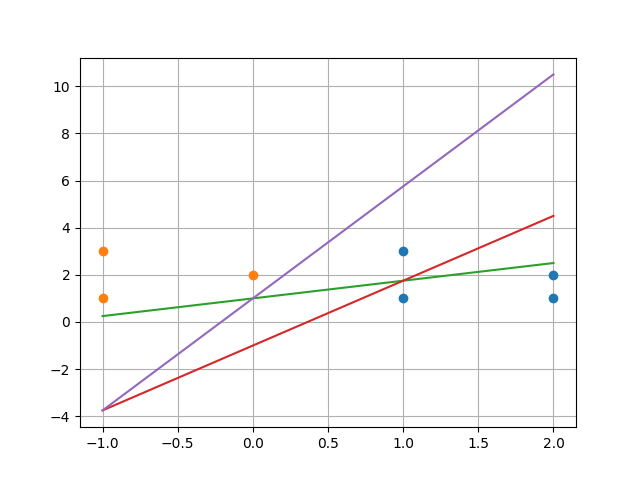
\includegraphics[width=0.75\textwidth]{simple-perceptron}
			\end{center}
			\caption{Evolución de los pesos conforme aumenta el número de iteraciones}
			\label{fig:e1_plot}
		\end{figure}

		\paragraph{}
		La figura \ref{fig:e1_plot} muestra la evolución del la recta que separa las dos clases de datos conforme aumentan las iteraciones. La línea en color \textbf{verde} se corresponde con la \textbf{iteración inicial}, la línea en color \textbf{verde} se corresponde con la \textbf{primera iteración} y, por último, la línea \textbf{púrpura} se corresponde con la \textbf{segunda iteración}. Nótese que en este punto las dos clases están separadas por dicha recta, por lo que el algoritmo ya está en codiciones de terminar.

		\begin{table}[h]
			\centering
			\small
			\begin{tabu}{ | c | c | }
				\hline
				\multicolumn{2}{ | c | }{Perceptrón Simple - Simple Dataset} \\ \hline
				Error de Resubstitucion & $0.0\%$	 \\
				\hline
			\end{tabu}
			\caption{Resultados del experimento sobre el conjunto de datos Simple}
			\label{table:e1_error}
		\end{table}

	\section{Adaline sobre Computer Hardware Dataset}
	\label{sec:e2}

		\paragraph{}
		En esta sección se describe el experimento realizado sobre el conjunto de datos \textbf{Computer Hardware}\cite{dataset:computer_hardware} y el algoritmo \textbf{Adaline}. Puesto que el algoritmo de aprendizaje realiza una regresión sobre los datos, para calcular la tasa de aciertos se ha utilizado como unidad de medida un \textbf{error relativo del $10\%$} sobre el valor real. Los parámetros utilizados para el ADALINE han sido un ratio de aprendizaje $\alpha = 0.1$ y $5000$ épocas.

		\paragraph{}
		La métodología experimental que se ha seguido ha sido un \textbf{HoldOut} con particionamiento de los datos de manera que $\frac{2}{3}$ son utilizados en la fase de entrenamiento y $\frac{1}{3}$ en la de test. Los resultados obtenidos tras dicha experimentación se recogen en la tabla \ref{table:e2_error}. Tal y como se puede apreciar, la tasa de error obtenida es muy elevada. Esto puede ser debido a la existencia de instancias muy diferentes unas de otras, lo cual penaliza drásticamente los resultados.


		\begin{table}[h]
			\centering
			\small
			\begin{tabu}{ | c | c | }
				\hline
				\multicolumn{2}{ | c | }{Adaline --- Computer Hardware Dataset} \\ \hline
				Error HoldOut & $71.429\%$	 \\
				\hline
			\end{tabu}
			\caption{[TODO ]}
			\label{table:e2_error}
		\end{table}

		\paragraph{}
		Tras realizar un experimento que utilizara todo el conjunto de datos (tanto para entrenamiento como para test) el error obtenido se redujo a $0.0\%$. Esta tarea se ha llevado a cabo para comprobar la corrección de la implementación utilizada. Sin embargo, nótese que esta circunstancia no es significativa para comprobar la validez del clasificador ADALINE sobre el conjunto de datos Computer Hardware puesto que en un entorno real esta situación no es posible.



%-----------------------------
%	Bibliographic references
%-----------------------------
	\nocite{subject:taa}
  \bibliographystyle{alpha}
  \bibliography{bib/misc}

\end{document}
